\hypertarget{setup-local-env}{%
\chapter{アプリケーション開発の準備}\label{setup-local-env}}
\thispagestyle{frontheadings}

これまでに学んだJavaScriptの基本構文は、実行環境を問わずに使えるものです。
しかしこの後に続くユースケースの章では、具体的な実行環境としてウェブブラウザと\href{https://nodejs.org/ja/}{Node.js}\footnote{\url{https://nodejs.org/ja/}}の2つを扱います。
また、ブラウザで実行するアプリケーションであっても、その開発にはツールとしてのNode.jsが欠かせません。
このセクションではユースケースの学習へ進むために必要なアプリケーション開発環境の準備をします。

\hypertarget{install-nodejs}{%
\section{Node.jsのインストール}\label{install-nodejs}}\index{Node.js}

\href{https://nodejs.org/ja/}{Node.js}はサーバーサイドJavaScript実行環境のひとつで、次のような特徴があります。

\begin{itemize}
\item
  ウェブブラウザのChromeと同じ\href{https://v8.dev/}{V8}\index{V8}
  JavaScriptエンジンで動作する
\item
  オープンソースで開発されている
\item
  OSを問わずクロスプラットフォームで動作する
\end{itemize}

Node.jsはサーバーサイドで使うために開発されました。
しかし今ではコマンドラインツールや\href{https://www.electronjs.org/}{Electron}\index{Electron}などのデスクトップアプリケーションにも利用されています。
そのため、Node.jsはサーバーサイドに限らずクライアントサイドのJavaScript実行環境としても幅広く使われています。

Node.jsは多くの他のプログラミング言語と同じように、実行環境をマシンにインストールすることで使用できます。
公式の\href{https://nodejs.org/ja/download/}{ダウンロードページ}\footnote{\url{https://nodejs.org/ja/download/}}から、開発用のマシンに合わせたインストーラをダウンロードして、インストールしましょう。

\begin{itemize}
\item ダウンロードページのURL: \href{https://nodejs.org/ja/download/}{\texttt{<https://nodejs.org/ja/download/>}}
\end{itemize}

Node.jsには\textbf{LTS(Long-Term
Support)}版\index{LTSばん@LTS版}\index{Node.js!LTSばん@LTS版}と最新版の2つのリリース版があります。 \textbf{LTS(Long-Term
Support)}版は2年間のメンテナンスとサポートが宣言されたバージョンです。
具体的には、後方互換性を壊さない範囲でのアップデートと、継続的なセキュリティパッチの提供が行われます。
一方で、最新版はNode.jsの最新の機能を使用できますが、常に最新のバージョンしかメンテナンスされません。
ほとんどのユーザーは、LTS版を用いることが推奨されます。Node.jsでの開発が初めてであれば、迷わずにLTS版のインストーラをダウンロードしましょう。
この章では執筆時点の最新LTS版であるバージョン18.14.0で動作するように開発します。

インストールが完了すると、コマンドラインで\texttt{node}\index{node@\texttt{node}}コマンドが使用可能になっているはずです。
次のコマンドを実行して、インストールされたNode.jsのバージョンを確認しましょう
(\texttt{\$}はコマンドラインの入力欄を表す記号であるため、実際に入力する必要はありません)。

\begin{lstlisting}
$ node -v
v18.14.0
\end{lstlisting}

また、Node.jsには\href{https://www.npmjs.com/}{npm}\index{npm}\footnote{\url{https://www.npmjs.com/}}というパッケージマネージャーが同梱されています。
Node.jsをインストールすると、\texttt{node}コマンドだけでなくnpmを扱うための\texttt{npm}\index{npm@\texttt{npm}}コマンドも使えるようになっています。
次のコマンドを実行して、インストールされたnpmのバージョンを確認しましょう。

\begin{lstlisting}
$ npm -v
9.3.1
\end{lstlisting}

Node.jsとnpmのバージョン番号は\texttt{\{major\}.\{minor\}.\{patch\}}という構成になっていて、先頭のメジャーバージョンが同じなら互換性は保証されています。

Node.jsのライブラリのほとんどはnpmを使ってインストールできます。
npmや\texttt{npm}コマンドについての詳細は\href{https://docs.npmjs.com/}{npmの公式ドキュメント}\footnote{\url{https://docs.npmjs.com/}}や\href{https://github.com/npm/cli}{npmのGitHubリポジトリ}\footnote{\url{https://github.com/npm/cli}}を参照してください。
実際に、ユースケースの章ではnpmを使ってライブラリをインストールして利用します。

\hypertarget{npx-execution}{%
\section{npxコマンドによるnpmパッケージの実行}\label{npx-execution}}

Node.jsを使ったコマンドラインツールは数多く公開されており、npmでインストールすることによりコマンドとして実行できるようになります。
ところで、Node.jsのインストールにより、\href{https://docs.npmjs.com/cli/v8/commands/npx/}{\texttt{npx}}\index{npx@\texttt{npx}}というコマンドも使えるようになっています。
\texttt{npx}コマンドを使うと、npmで公開されている実行可能なパッケージのインストールと実行をまとめてできます。
この後のユースケースでも\texttt{npx}コマンドでツールを利用するため、ここでツールの実行を試してみましょう。

ここでは例として\href{https://github.com/js-primer/hello-world}{\texttt @js-primer/hello-world}というサンプル用のパッケージを実行します。
\texttt{npx}コマンドでコマンドラインツールを実行するには、次のように
\texttt{npx}コマンドにパッケージ名を渡して実行します。
npx 7から、初めて実行するコマンドは対話式のプロンプトでパッケージをインストールするかが確認されます。
このプロンプトに対して\keytop{Enter}キーを押すとインストールが開始され、コマンドが実行されます。

\begin{lstlisting}[escapechar=\*]
$ npx @js-primer/hello-world
Need to install the following packages:
  @js-primer/hello-world@1.0.0
Ok to proceed? (y)
# 初回は@js-primer/hello-worldをインストールしていいかを確認するプロンプトが表示される
# *\keytop{Enter}*を押すとインストールが開始され、コマンドが実行される

Hello World!
\end{lstlisting}

デフォルトでは対話式のプロンプトが挟まれますが、次のように\texttt{-\/-yes}オプションを付与すると自動的にインストールとコマンドが実行されます。

\begin{lstlisting}
# --yesオプションで、インストールの確認プロンプトをスキップする
$ npx --yes @js-primer/hello-world
Hello World!
\end{lstlisting}

このように、\texttt{npx}コマンドを使うことによりnpmで公開されているコマンドラインツールを簡単に実行できます。

\begin{tcolorbox}[title=コマンドラインツールのインストールと実行]\label{command-line-tools-installation}\index{こまんどらいんつーる@コマンドラインツール}

npmで公開されているコマンドラインツールを実行する方法は\texttt{npx}コマンドだけではありません。
\texttt{npm install}コマンドを使ってパッケージをインストールし、インストールされたパッケージのコマンドを実行する方法があります。
通常の\texttt{npm install}コマンドは実行したカレントディレクトリにパッケージをインストールしますが、\texttt{-\/-global}\index{--global@\texttt{-\/-global}}フラグを加えるとパッケージをグローバルインストールします。
グローバルインストールされたパッケージのコマンドは、\texttt{node}コマンドや\texttt{npm}コマンドと同じように、任意の場所から実行できます。

次の例では\texttt{@js-primer/hello-world}パッケージをグローバルインストールしています。
その後、パッケージに含まれている\texttt{js-primer-hello-world}コマンドを絶対パスの指定なしで呼び出しています。

\begin{lstlisting}
$ npm install --global @js-primer/hello-world
$ js-primer-hello-world
Hello World!
\end{lstlisting}
\end{tcolorbox}

\hypertarget{local-server}{%
\section{ローカルサーバーのセットアップ}\label{local-server}}\index{ろーかるさーばー@ローカルサーバー}

「\hyperlink{read-eval-print}{値の評価と表示}」の章では、\texttt{index.html}と\texttt{index.js}というファイルを作成してブラウザで表示していました。
このときローカルに作成したHTMLファイルをそのままブラウザで読み込むと、ブラウザのアドレスバーは\texttt{file:///}からはじまるURLになります。
\texttt{file}スキーマ\index{fileすきーま@\texttt{file}スキーマ}では\href{https://developer.mozilla.org/ja/docs/Web/Security/Same-origin_policy}{Same Origin
Policy}\index{Same Origin Policy}\footnote{\url{https://developer.mozilla.org/ja/docs/Web/Security/Same-origin_policy}}というセキュリティ的な制限により、多くの場面でアプリケーションは正しく動作しません。

これからユースケースの章で書いていくアプリケーションは、\href{https://developer.mozilla.org/ja/docs/Web/Security/Same-origin_policy}{Same Origin
Policy}の制限を避けるために、\texttt{http}スキーマ\index{httpすきーま@\texttt{http}スキーマ}のURLでアクセスすることを前提としています。
開発用のローカルサーバーを使うことで、ローカルに作成したHTMLファイルも\texttt{http}スキーマのURLで表示できます。

ここでは、これからのユースケースで利用する開発用のローカルサーバーをセットアップする方法を見ていきます。

\hypertarget{preparing-html}{%
\subsection{HTMLファイルの用意}\label{preparing-html}}\index{HTMLふぁいる@HTMLファイル}

まずは最低限の要素だけを配置したHTMLファイルを作成しましょう。
ここでは\texttt{index.html}というファイル名で作成し、HTMLファイル内には次のように記述しています。
このHTMLファイルでは\texttt{script}\index{script@\texttt{script}}要素を使って\texttt{index.js}というファイル名のJavaScriptファイルを読み込んでいます。

\begin{listtitle}
index.html
\end{listtitle}
\begin{lstlisting}
<!DOCTYPE html>
<html lang="ja">
  <head>
    <meta charset="utf-8" />
    <title>Ajax Example</title>
  </head>
  <body>
    <h2>GitHub User Info</h2>
    <script src="index.js"></script>
  </body>
</html>
\end{lstlisting}
\listend


同じように\texttt{index.js}というファイル名でJavaScriptファイルを作成します。
この\texttt{index.js}には、スクリプトが正しく読み込まれたことを確認できるよう、コンソールにログを出力する処理だけを書いておきます。

\begin{listtitle}
index.js
\end{listtitle}
\begin{lstlisting}
import { App } from "./src/App.js";
const app = new App();
\end{lstlisting}
\listend


\hypertarget{open-js-primer-local-server}{%
\subsection{ローカルサーバーを起動する}\label{open-js-primer-local-server}}\index{ろーかるさーばー@ローカルサーバー!きどう@起動}

先ほど作成した\texttt{index.html}と同じディレクトリで、ローカルサーバーを起動します。
次のコマンドでは、\href{https://github.com/js-primer/local-server}{\texttt{@js-primer/local-server}}というこの書籍用に作成されたローカルサーバーモジュールをダウンロードと同時に実行します。
このローカルサーバーモジュールは、\texttt{http}スキーマのURLでローカルファイルへアクセスできるように、実行したディレクトリにあるファイルを配信する機能を持ちます。

\begin{lstlisting}
# からはじまる行はコメントなので実行はしなくてよい
# cdコマンドでファイルがあるディレクトリまで移動
$ cd "index.htmlがあるディレクトリのパス"

# npx コマンドでローカルサーバーを起動
$ npx --yes @js-primer/local-server

js-primerのローカルサーバーを起動しました。
次のURLをブラウザで開いてください。

  URL: http://localhost:3000
\end{lstlisting}

起動したローカルサーバーのURL(\texttt{http://localhost:3000})へブラウザでアクセスすると、先ほどの\texttt{index.html}の内容が表示されます。
多くのサーバーでは、\texttt{http://localhost:3000}のようにファイルパスを指定せずにアクセスすると、\texttt{index.html}を配信する機能を持っています。
\texttt{@js-primer/local-server}もこの機能を持つため、\texttt{http://localhost:3000}と\texttt{http://localhost:3000/index.html}のどちらのURLも同じ\texttt{index.html}を配信しています。

\begin{figure}[h]
\centering
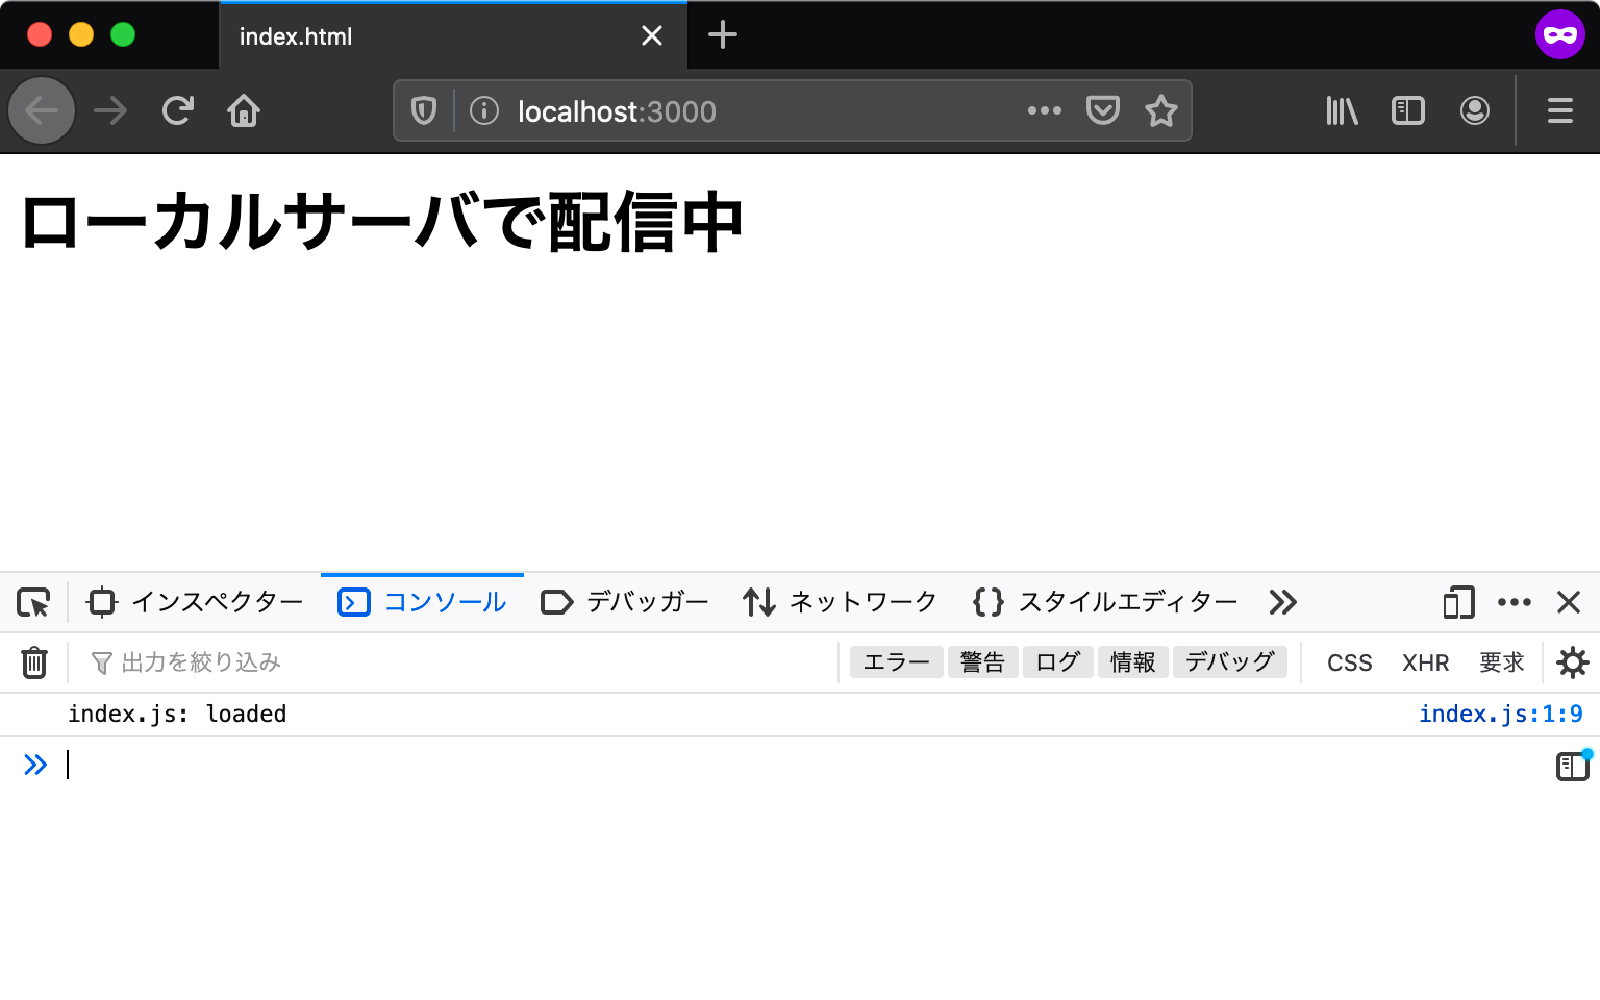
\includegraphics[width=120mm]{fig/index.pdf}
\caption{ログが表示されているウェブコンソール}
\end{figure}

\texttt{index.html}にアクセスできたら、正しく\texttt{index.js}が読み込まれているかを確認してみましょう。
Console
APIで出力したログを確認するには、ウェブブラウザの開発者ツールを開く必要があります。
ほとんどのブラウザで開発者ツールが同梱されていますが、この書籍ではFirefoxを使って確認します。

Firefox\index{Firefox}の開発者ツール\index{かいはつしゃつーる@開発者ツール}は次のいずれかの方法で開きます。

\begin{itemize}
\item
  Firefoxメニュー(メニューバーがある場合やmacOS
  では、ツールメニュー)の``ブラウザーツール''のサブメニューから``ウェブ開発ツール''
  を選択する
\item
  キーボードショートカット\keytop{Ctrl}+\keytop{Shift}+\keytop{K}(macOSでは
  \keytop{Command}+\keytop{Option}+\keytop{K})を押下する
\end{itemize}

詳細は\href{https://developer.mozilla.org/ja/docs/Learn/Common_questions/What_are_browser_developer_tools}{「ブラウザーの開発者ツールとは?」}\footnote{\url{https://developer.mozilla.org/ja/docs/Learn/Common_questions/What_are_browser_developer_tools}}を参照してください。

\hypertarget{close-js-primer-local-server}{%
\subsection{ローカルサーバーを終了する}\label{close-js-primer-local-server}}\index{ろーかるさーばー@ローカルサーバー!しゅうりょう@終了}

最後に、起動したローカルサーバーを終了します。
ローカルサーバーを起動したコマンドラインで、\keytop{Ctrl}+\keytop{C}を押下することで終了できます。

複数のローカルサーバーを同時に起動することもできますが、複数のサーバーで同じポート番号\index{ぽーとばんごう@ポート番号}を利用することはできません。
ポートとは、先ほど起動したローカルサーバーのURLで\texttt{:3000}となっていた部分のことで、これは3000番ポートでローカルサーバーを起動したことを意味しています。

\texttt{@js-primer/local-server}は、デフォルトのポート(3000番ポート)がすでに使用されているなら、使われていないポートを探してローカルサーバーを起動します。また、\texttt{-\/-port}\index{--port@\texttt{-\/-port}}オプションで任意のポート番号でローカルサーバーを起動できます。

\begin{lstlisting}
$ npx --yes @js-primer/local-server --port 8000
\end{lstlisting}

この書籍では、\texttt{@js-primer/local-server}をデフォルトのポート番号である3000番ポートを利用する前提で進めていきます。
使わなくなったローカルサーバーは\keytop{Ctrl}+\keytop{C}で終了しておくことで、アクセスするURL(ポート番号)が書籍と同じ状態で進められます。

\hypertarget{conclusion}{%
\section{まとめ}\label{conclusion}}

この章では、これからのユースケースの章で必要な環境を準備しました。

\begin{itemize}
\item
  Node.jsのLTS版をインストールした
\item
  npmとnpxでモジュールのインストールと実行をした
\item
  \texttt{@js-primer/local-server}モジュールを使ってローカルサーバーを起動して終了した
\end{itemize}

npmでは、すでに多種多様なローカルサーバーモジュールが公開されています。
この書籍では、利用するローカルサーバーの機能で違いが出ないように\texttt{@js-primer/local-server}というこの書籍用のローカルサーバーモジュールを利用します。
